\documentclass{article}
\usepackage[utf8]{inputenc}
\usepackage{amsmath,amssymb,amsthm,mathrsfs,graphicx}
\usepackage{float}

\title{HW7}
\author{Ry Wiese\\wiese176@umn.edu}
\date{November 22, 2019}

\begin{document}

\maketitle

\section{Problem 1}

\subsection{Part 1}

False. 
Let $f(x) = - ln(x)$ and $g(x) = e^{x^2}$. Both $f$ and $g$ are convex. However, $(f \circ g)(x) = -ln(e^{x^2}) = -x^2$ is concave. 

\subsection{Part 2}

True.

\begin{proof}

Assume $f$ is convex and nondecreasing. Assume $g$ is convex.\\
Let $\mu_1, \mu_2 \in dom[f \circ g]$ be given, and let $\lambda$ be given with $0 < \lambda < 1$.\\
Since $g$ is convex, $g(\lambda \mu_1 + (1 - \lambda) \mu_2) \le \lambda g(\mu_1) + (1 - \lambda) g(\mu_2).$\\
Therefore, since $f$ is non-decreasing,\\ $f(g(\lambda \mu_1 + (1 - \lambda) \mu_2)) \le f(\lambda g(\mu_1) + (1 - \lambda) g(\mu_2))$.\\
Since $f$ is convex, $f(\lambda g(\mu_1) + (1 - \lambda) g(\mu_2)) \le \lambda f(g(\mu_1)) + (1 - \lambda) f(g(\mu_2))$.\\
Putting this together, we have\\
$(f \circ g)(\lambda \mu_1 + (1 - \lambda) \mu_2) = f(g(\lambda \mu_1 + (1 - \lambda) \mu_2)) \le f(\lambda g(\mu_1) + (1 - \lambda) g(\mu_2)) \le \lambda f(g(\mu_1)) + (1 - \lambda) f(g(\mu_2)) = \lambda (f \circ g) (\mu_1) + (1 - \lambda) (f \circ g) (\mu_2)$.\\
Thus $f \circ g$ is convex.

\end{proof}

\subsection{Part 3}

False.
Let $f(x) = -e^x$ and let $g(x) = x^2$. $f$ is concave and non-increasing, $g$ is convex, but $(f \circ g)(x) = - e^{x^2}$ is concave. 

\subsection{Part 4}

True. I'm struggling to come up with a formal proof. However, it seems to me that $x \cdot f(x)$ is asymptotically bound below by the function $x$, which is convex, and that since $f(x)$ is non-negative and non-decreasing, $x \cdot f(x)$ would have to curve upward at a rate faster than $x$ which would make it also convex.

\subsection{Part 5}

True.
$\frac{d}{dx}(-log(-f(x))) = - \frac{1}{|-f(x)|} \cdot - f'(x) = - f(x)^{-1} f'(x)$ since $f(x) < 0$.\\
$\frac{d^2}{dx^2}(-log(-f(x))) = \frac{d}{dx}(- f(x)^{-1} f'(x)) = -[\frac{d}{dx}(f(x)^{-1}) \cdot f'(x) + f(x)^{-1} \cdot \frac{d}{dx}(f'(x))] = \frac{f'(x)^2}{f(x)^2} - \frac{f''(x)}{f(x)} = \frac{f'(x)^2 - f(x) \cdot f''(x)}{f(x)^2} \ge 0$, since $f'(x)^2 \ge 0$, $f(x)^2 \ge 0$, and $-f(x) \cdot f''(x) \ge 0$ (since $f(x) < 0$ and since $f$ is convex $\therefore f''(x) \ge 0$).

\section{Problem 2}

\subsection{Part 1}

Denote the Hessian of $f$ as $H$ where $H = \left( \begin{array}{cc} \frac{\partial^2 f}{\partial x_1^2} & \frac{\partial^2 f}{\partial x_1 \partial x_2}\\ \frac{\partial^2 f}{\partial x_1 \partial x_2} & \frac{\partial^2 f}{\partial x_2^2} \end{array} \right) = \left( \begin{array}{cc} \frac{e^{x_1 + x_2}}{(e^{x_1} + e^{x_2})^2} & \frac{-e^{x_1 + x_2}}{(e^{x_1} + e^{x_2})^2}\\ \frac{-e^{x_1 + x_2}}{(e^{x_1} + e^{x_2})^2} & \frac{e^{x_1 + x_2}}{(e^{x_1} + e^{x_2})^2} \end{array} \right)$.
The determinants of the principal submatrices of $H$ are\\
$$det(H_1) = \frac{e^{x_1 + x_2}}{(e^{x_1} + e^{x_2})^2} \ge 0$$
and
$$det(H_2) = (\frac{e^{x_1 + x_2}}{(e^{x_1} + e^{x_2})^2})^2 - (\frac{-e^{x_1 + x_2}}{(e^{x_1} + e^{x_2})^2})^2 = 0 \ge 0$$
The determinants of all principal submatrices are non-negative, so $H$ is a PSD matrix. Thus $f$ is convex.

\subsection{Part 2}

\[
\begin{array}{rrclcc}
 \min & e^{a - b} &      &   \\
 \mbox{s.t.}  &  -10  & \le  & a & \le & 3 ~; \\
    & e^{2a - \frac{b}{2}} & + & e^{\frac{b}{2} - c} & \le & 1;\\
    &&& a - b & = & 2c
 \end{array}
\]

\subsection{Part 3}

I got an optimal solution of $x = e^{-10}$, $y = e^{-5}$, and $z = e^{-2.5}$ and an optimal value of 0.00673795. This can be reproduced by running the Matlab file P3.m.

\section{Problem 3}

\subsection{Part 1}

\begin{figure}[H] % "h" is where to place, h=here, t=top, b=bottom
  \centering
  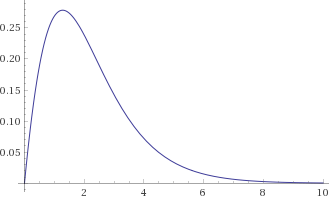
\includegraphics[angle=0,totalheight=50mm]{P3.png}
  \caption{Graph of $r(p)$}
  \label{fig:tabl}
\end{figure}

Let $u_1 = 4$ and let $u_2 = 8$. Let $l(p)$ be the line segment connecting $r(u_1)$ and $r(u_2)$. We can clearly see that, for all points $p_0$ along the line segment between $u_1$ and $u_2$, $r(p_0) \le l(p_0)$. Thus $r$ is not concave.

\subsection{Part 2}

$$\lambda = \frac{e^{-p}}{1 + e^{-p}}$$
$$\lambda (1 + e^{-p}) = e^{-p}$$
$$\lambda + \lambda e^{-p} = e^{-p}$$
$$\lambda e^p + \lambda = 1$$
$$\lambda e^p = 1 - \lambda$$
$$e^p = \frac{1 - \lambda}{\lambda}$$
$$p = ln(\frac{1 - \lambda}{\lambda})$$

$p \lambda(p) = ln(\frac{1 - \lambda}{\lambda}) \cdot \lambda$\\

\begin{figure}[H] % "h" is where to place, h=here, t=top, b=bottom
  \centering
  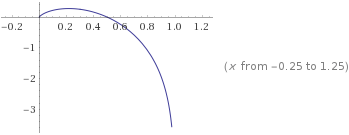
\includegraphics[angle=0,totalheight=50mm]{P33.png}
  \caption{Graph of $r(\lambda)$}
  \label{fig:tabl}
\end{figure}

Clearly, this function is concave. 

\subsection{Part 3}

\subsubsection{Main Condition}

$$\frac{1}{\lambda - 1} + ln(\frac{1}{\lambda} - 1) + \eta_1 - \eta _2 = 0$$

\subsubsection{Dual Feasibility}

$$\eta_1, \eta_2 \ge 0$$

\subsubsection{Complementarity}

$$\eta_1(\lambda - 1) = 0$$
$$\eta(-\lambda) = 0$$

\subsubsection{Primal Feasibility}

$$0 \le \lambda \le 1$$

\subsubsection{Transformed Main Condition}

$$\frac{1}{\frac{e^{-p}}{1 + e^{-p}} - 1} + ln(\frac{1}{\frac{e^{-p}}{1 + e^{-p}}} - 1) + \eta_1 - \eta _2 = 0$$

\subsubsection{Transformed Dual Feasibility}

$$\eta_1, \eta_2 \ge 0$$

\subsubsection{Transformed Complementarity}

$$\eta_1(\frac{e^{-p}}{1 + e^{-p}} - 1) = 0$$
$$\eta(-\frac{e^{-p}}{1 + e^{-p}}) = 0$$

\subsubsection{Transformed Primal Feasibility}

$$0 \le \frac{e^{-p}}{1 + e^{-p}} \le 1$$



\section{Problem 4}

The two roots I found were 1.7000 and 5.4069. This can be reproduced by running the Matlab file P4.m.

\end{document}
